\documentclass[10pt]{beamer}
\usepackage{amsmath}
\usepackage{amssymb}
\usepackage{geometry}
\usepackage{graphicx}
\usepackage{url}

% some latex magic for correcting apostrophe issue in verbatim mode
\makeatletter
\let \@sverbatim \@verbatim
\def \@verbatim {\@sverbatim \verbatimplus}
{\catcode`'=13 \gdef \verbatimplus{\catcode`'=13 \chardef '=13 }} 
\makeatother


\begin{document}

%---------------------------------------------
\begin{frame}
\large
Lab 3: Intro to Data Visualization\\
STAT 630, Fall 2021
\vspace{15pt}

\normalsize
Topics:
\begin{itemize}
\item Tables
\item Contingency Tables
\item Bar Plots
\item Histograms
\item Maps
\end{itemize}
\end{frame}

%----------------------------------------------
\begin{frame}[fragile]{Tables}
\begin{verbatim}
# frequency table
> table(cdc$smoke100)
    0     1 
10559  9441 

# relative frequency table
> table(cdc$smoke100) / 20000
      0       1 
0.52795 0.47205 
\end{verbatim}
\end{frame}

%----------------------------------------------
\begin{frame}[fragile]{Bar Plots}
\small
\begin{verbatim}
> smoke_tb <- table(cdc$smoke100)
> barplot(smoke_tb, xlab="Smoked at least 100 cigarettes", 
          names.arg = c("no", "yes"), ylab="Count") 
> barplot(smoke_tb/20000, xlab="Smoked at least 100 cigarettes", 
          names.arg = c("no", "yes"), ylab="Proportion")
\end{verbatim}
\normalsize

\begin{figure}[htbp]
\centering
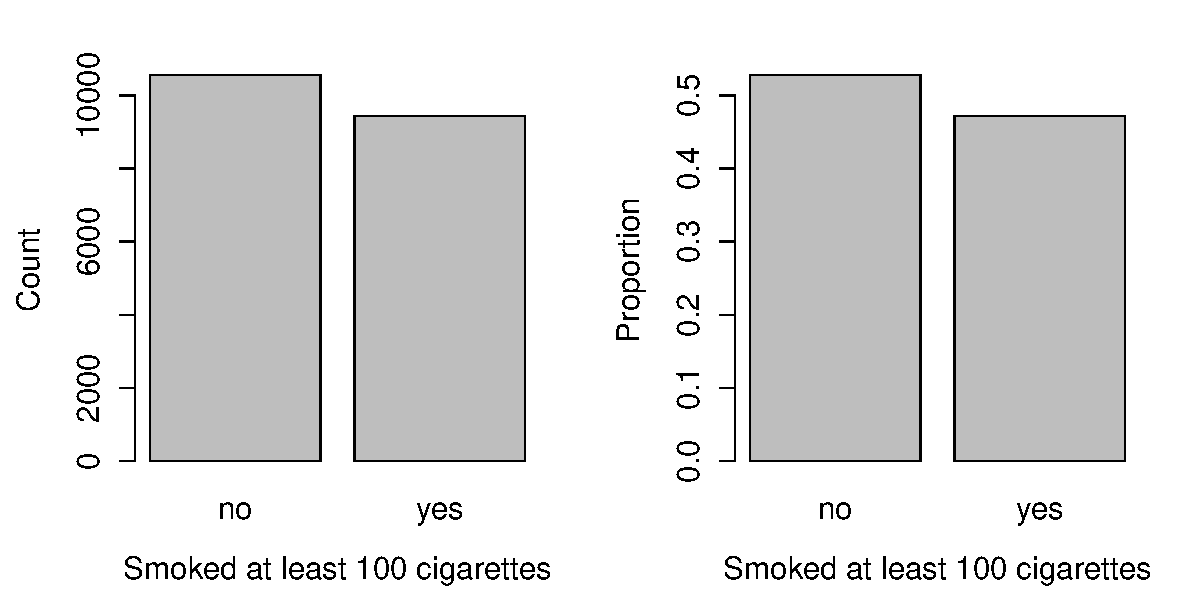
\includegraphics[width=0.8\textwidth]{figure/barplot_smoke.pdf}
\end{figure}
\end{frame}

%----------------------------------------------
\begin{frame}[fragile]{Contingency Tables}
\begin{verbatim}
> table(cdc$smoke100, cdc$gender)

       f    m
  0 6012 4547
  1 4419 5022
  
> addmargins(table(cdc$smoke100, cdc$gender))

          f     m   Sum
  0    6012  4547 10559
  1    4419  5022  9441
  Sum 10431  9569 20000
\end{verbatim}
\end{frame}

%----------------------------------------------
\begin{frame}[fragile]{Stacked Bar Plot}
\begin{verbatim}
> barplot(table(cdc$smoke100, cdc$gender), 
          col=c("grey", "cyan"))
> legend("bottomright", c("no", "yes"), col=c("grey", "cyan"), 
         title="smoke", pch=16)
\end{verbatim}

\begin{figure}[htbp]
\centering
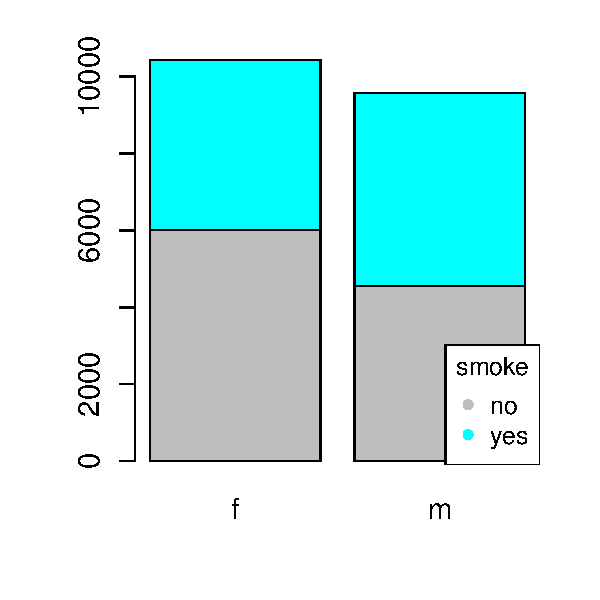
\includegraphics[scale=0.5]{figure/barplot_smokegen_stacked.pdf}
\end{figure}
\end{frame}


%----------------------------------------------
\begin{frame}[fragile]{Row and Column Proportions}
\begin{verbatim}
> prop.table(table(cdc$smoke100, cdc$gender))
          f       m
  0 0.30060 0.22735
  1 0.22095 0.25110 

# divides counts by row totals  
> prop.table(table(cdc$smoke100, cdc$gender), margin=1)  
            f         m
  0 0.5693721 0.4306279
  1 0.4680648 0.5319352
  
# divides counts by column totals  
> prop.table(table(cdc$smoke100, cdc$gender), margin=2) 
            f         m
  0 0.5763589 0.4751803
  1 0.4236411 0.5248197
\end{verbatim}
\end{frame}

%----------------------------------------------
\begin{frame}[fragile]
\small
\begin{verbatim}
> proptb <- prop.table(table(cdc$smoke100, cdc$gender), margin=2)
> barplot(proptb, col=c("grey", "cyan"), ylab="Proportion")
> legend("bottomright", c("no", "yes"), col=c("grey", "cyan"), 
         title = "smoke", pch=16)
\end{verbatim}
\begin{figure}[htbp]
\centering
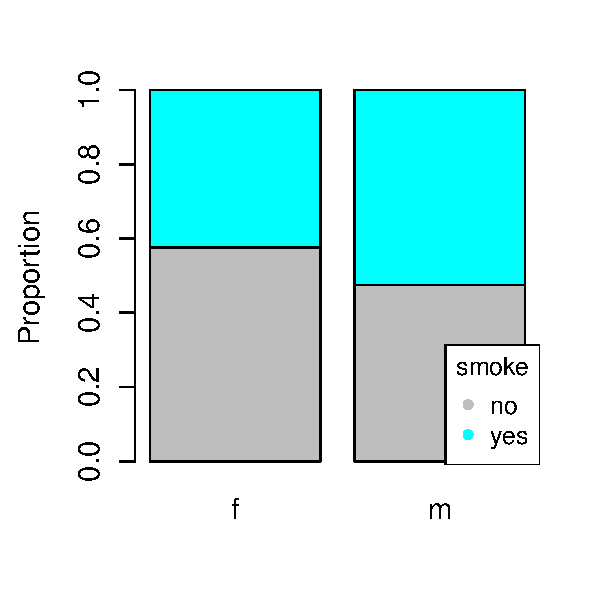
\includegraphics[scale=0.5]{figure/barplot_smokegen_prop.pdf}
\end{figure}
\end{frame}

%----------------------------------------------
\begin{frame}{Factors}
\begin{itemize}
\item Categorical data in R is often represented as a data type called a \textbf{factor}.
\vspace{5pt}
\item Specifically, factors are stored as integers that have labels associated with each unique integer value.  The labels are the names of the different categories.
\vspace{5pt}
\item Use the \texttt{factor()} function to create a factor, and the \texttt{levels} argument to specify the ordering of the categories.
\end{itemize}
\end{frame}

%----------------------------------------------
\begin{frame}[fragile]
\small
\begin{verbatim}
> class(cdc$genhlth)
[1] "character"

> table(cdc$genhlth)
excellent      fair      good      poor very good 
     4657      2019      5675       677      6972 

# create factor and specify order for levels  
> cdc$genhlth <- factor(cdc$genhlth, 
    levels=c("poor", "fair", "good", "very good", "excellent"))
    
> class(cdc$genhlth)
[1] "factor"

> table(cdc$genhlth)
     poor      fair      good very good excellent 
      677      2019      5675      6972      4657 
\end{verbatim}
\end{frame}

%----------------------------------------------
\begin{frame}[fragile]
\small
\begin{verbatim}
> barplot(table(cdc$genhlth), xlab="General health", ylab="Count")
\end{verbatim}
\begin{figure}[htbp]
\centering
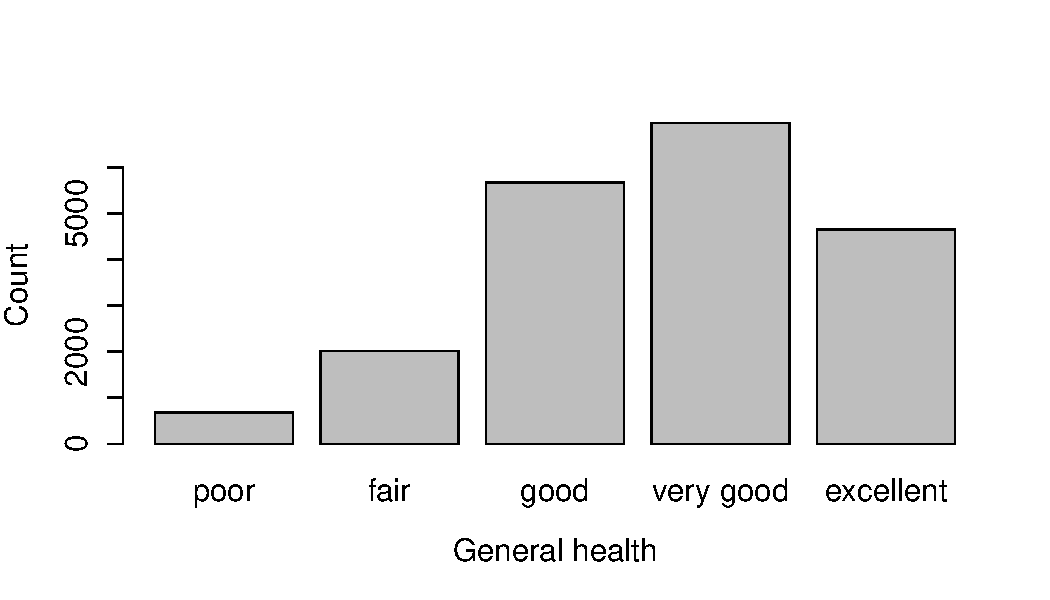
\includegraphics[width=0.8\textwidth]{figure/barplot_genhealth.pdf}
\end{figure}
\end{frame}

%----------------------------------------------
% \begin{frame}[fragile]
% Using a factor instead of a character vector makes it obvious when some categories contain no observations.
% \begin{verbatim}
% > gender_char <- c("m", "m", "m")
% > table(gender_char)
% gender_char
% m
% 3
% 
% > gender_factor <- factor(gender_char, levels=c("m", "f"))
% > table(gender_factor)
% gender_factor
% m f
% 3 0
% \end{verbatim}
% \end{frame}

%----------------------------------------------
\begin{frame}{\texttt{ggplot2}}
\texttt{ggplot2} is a popular R package for data visualization.  It was created by Hadley Wickham.\\
\vspace{3pt}
Reference: \url{https://ggplot2.tidyverse.org}
\vspace{15pt}

In this class, so far we have focus on the base R approach to creating graphics (the original plotting system in R).  I think it's important to know both approaches, since each has its advantages -- base R graphics tend to be more customizable, while \texttt{ggplot2} graphics tend to look nicer without many adjustments. The \texttt{ggplot2} approach also has some advantages when dealing with categorical data.\\
\end{frame}

%---------------------------------------
\begin{frame}[fragile]
To install \texttt{ggplot2} run the following command in the console:
\begin{verbatim}
> install.packages("ggplot2")
\end{verbatim}
You only need to install the package once. (If you are using the R Studio Cloud, you don't need to do this since the package should already be installed.)\\
\vspace{20pt}

To load \texttt{ggplot2} into your current R session run the following command:
\begin{verbatim}
> library(ggplot2)
\end{verbatim}
This command needs to be run during each R session when you use the package. 
\end{frame}


%---------------------------------------
\begin{frame}[fragile]
\begin{verbatim}
library(ggplot2)
ggplot(data = cdc) + 
  geom_bar(aes(x=genhlth)) +
  labs(x="general health")
\end{verbatim}
\begin{figure}[htbp]
\centering
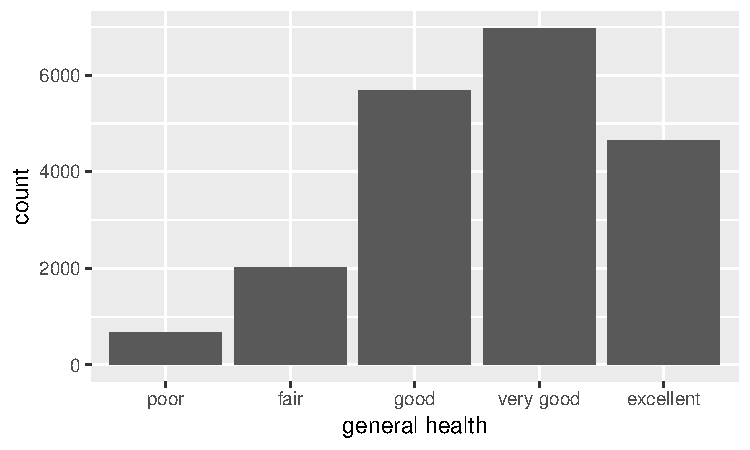
\includegraphics[scale=0.6]{figure/barplot_hlth_gg.pdf}
\end{figure}
\end{frame}

%---------------------------------------
\begin{frame}[fragile]
\begin{verbatim}
ggplot(data = cdc) + 
  geom_bar(aes(x=genhlth, fill=factor(smoke100))) + 
  labs(x="general health", fill="smoke")
\end{verbatim}
\begin{figure}[htbp]
\centering
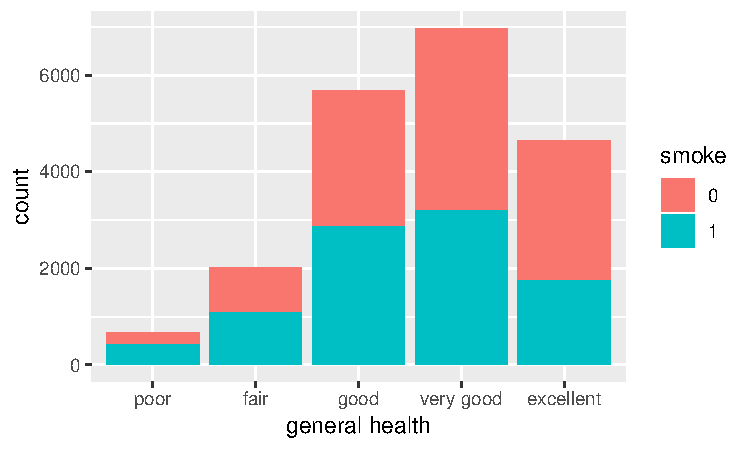
\includegraphics[scale=0.6]{figure/barplot_stack_hlthsmoke_gg.pdf}
\end{figure}
\end{frame}

%---------------------------------------
\begin{frame}[fragile]
\small
\begin{verbatim}
ggplot(data = cdc) +
  geom_bar(aes(x=genhlth, fill=factor(smoke100)), position="dodge") + 
  labs(x="general health", fill="smoke")
\end{verbatim}
\begin{figure}[htbp]
\centering
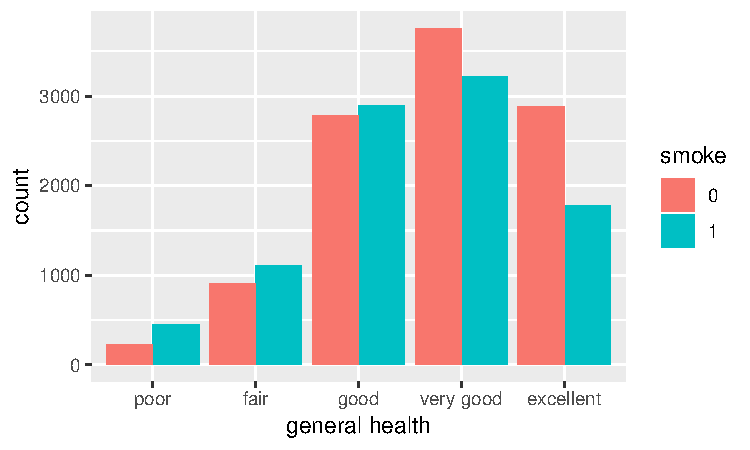
\includegraphics[scale=0.6]{figure/barplot_side_hlthsmoke_gg.pdf}
\end{figure}
\end{frame}

%---------------------------------------
\begin{frame}[fragile]
\small
\begin{verbatim}
ggplot(data = cdc) + 
  geom_bar(aes(x=genhlth, fill=factor(smoke100)), position="fill") + 
  labs(x="general health", y="proportion", fill="smoke")
\end{verbatim}
\begin{figure}[htbp]
\centering
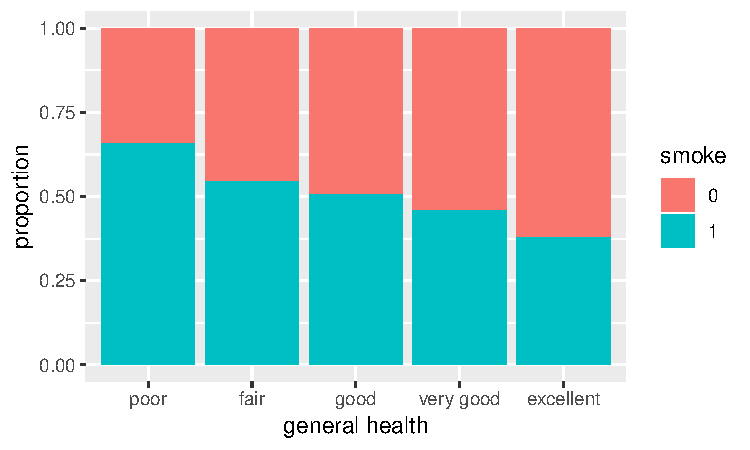
\includegraphics[scale=0.6]{figure/barplot_prop_hlthsmoke_gg.pdf}
\end{figure}
\end{frame}

%---------------------------------------
\begin{frame}[fragile]{Histograms}
\begin{itemize}
\item Histograms are a useful way to visualize the distribution of a numerical (continuous) variable.
\vspace{5pt}
\item To construct a histogram, the range of the data is divided into bins of equal width.  Then the number of observations falling in each bin are counted.  The counts are plotted as rectangles over each bin.
\end{itemize}
\end{frame}

%---------------------------------------
\begin{frame}[fragile]
\small
\begin{verbatim}
> sort(mtcars$mpg)
 [1] 10.4 10.4 13.3 14.3 14.7 15.0 15.2 15.2 15.5 15.8 16.4
[12] 17.3 17.8 18.1 18.7 19.2 19.2 19.7 21.0 21.0 21.4 21.4
[23] 21.5 22.8 22.8 24.4 26.0 27.3 30.4 30.4 32.4 33.9
\end{verbatim}

\begin{tabular}{l|lllll}
Bin & $(10, 15]$ & $(15, 20]$ & $(20, 25]$ & $(25, 30]$ & $(30,35]$\\
\hline
Count & 6 & 12 & 8 & 2 & 4\\
\end{tabular}

\begin{verbatim}
> hist(mtcars$mpg, main='', xlab="Miles per gallon (mpg)")
\end{verbatim}

\begin{figure}[htbp]
\centering
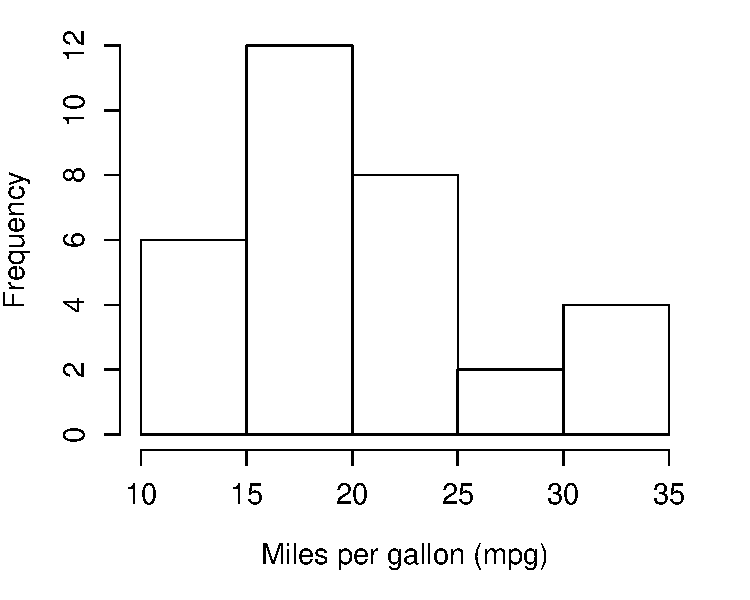
\includegraphics[width=0.5\textwidth]{figure/hist_mpg1.pdf}
\end{figure}
\end{frame}

%---------------------------------------
% \begin{frame}[fragile]{Attributes}
% \small
% \begin{verbatim}
% > h1 <- hist(mtcars$mpg)
% 
% > attributes(h1)
% $names
% [1] "breaks"   "counts"   "density"  "mids"     "xname"    "equidist"
% 
% $class
% [1] "histogram"
% 
% > h1$breaks
% [1] 10 15 20 25 30 35
% 
% > h1$counts
% [1]  6 12  8  2  4
% \end{verbatim}
% \end{frame}

%---------------------------------------
\begin{frame}[fragile]
\footnotesize
\begin{verbatim}
> par(mfrow=c(2,2)) # split plot into 4 panels
> hist(cdc$weight, main="default # of bins")
> hist(cdc$weight, breaks=10, main="10 bins")
> hist(cdc$weight, breaks=50, main="50 bins")
> hist(cdc$weight, breaks=100, main="100 bins")
> dev.off() # resets graphical parameters
\end{verbatim}
\begin{figure}[htbp]
\centering
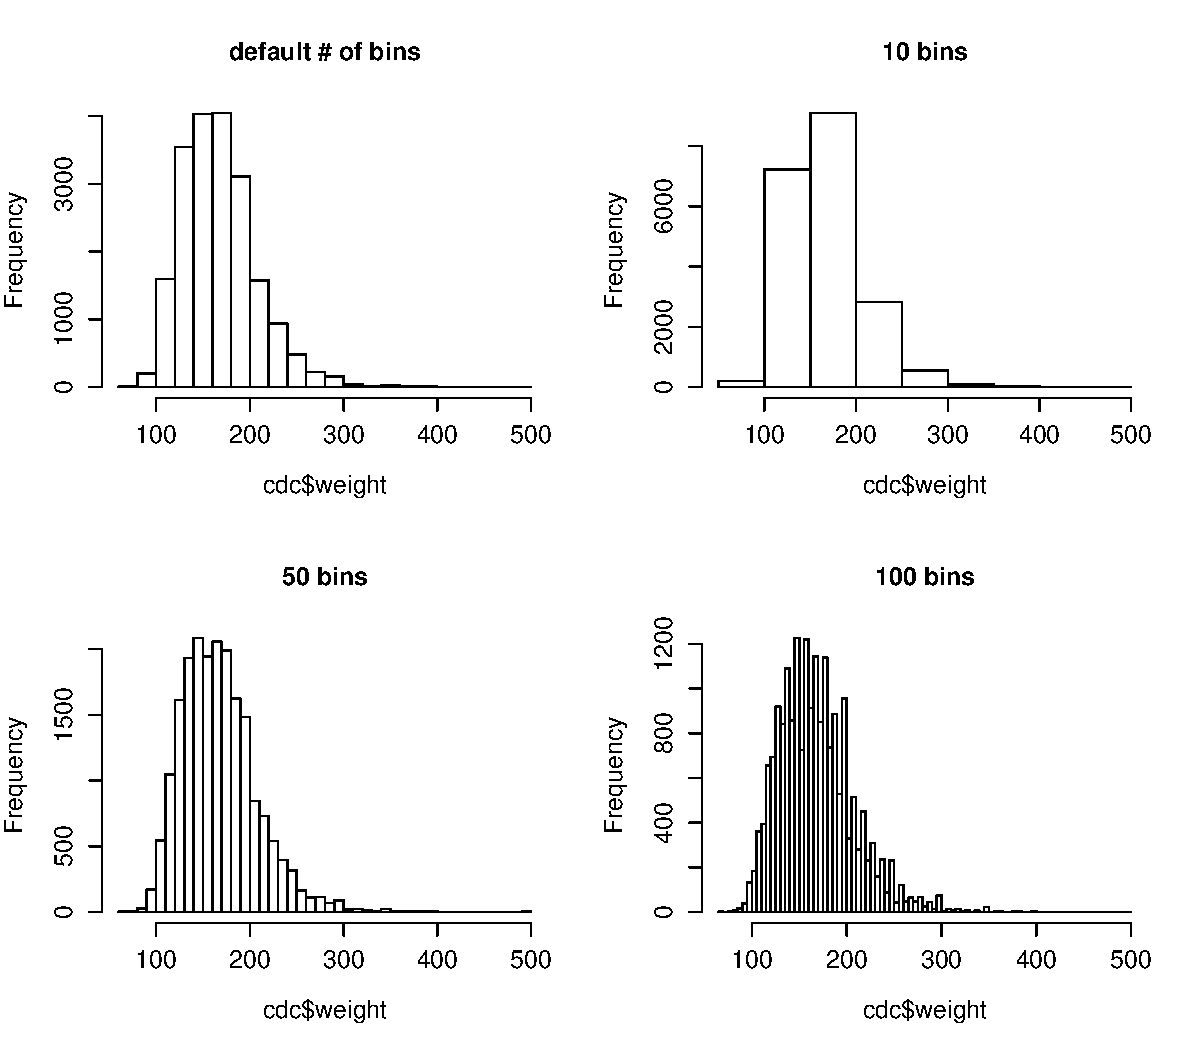
\includegraphics[width=0.75\textwidth]{figure/hist_weight_bins.pdf}
\end{figure}
\end{frame}

%------------------------------
% \begin{frame}[fragile]{Histogram Density Plot}
% \begin{itemize}
% \item To make a histogram density plot set \texttt{freq=FALSE}
% \item When density values are plotted the area under the histogram is 1 (i.e., integrates to 1).  Note that the area under a histogram is computed by summing up the areas of each rectangle (bin widths $\times$ heights)
% \end{itemize}
% \begin{verbatim}
% > hist(mtcars$mpg, freq=FALSE, main='')
% \end{verbatim} 
% \begin{figure}[htbp]
% \centering
% 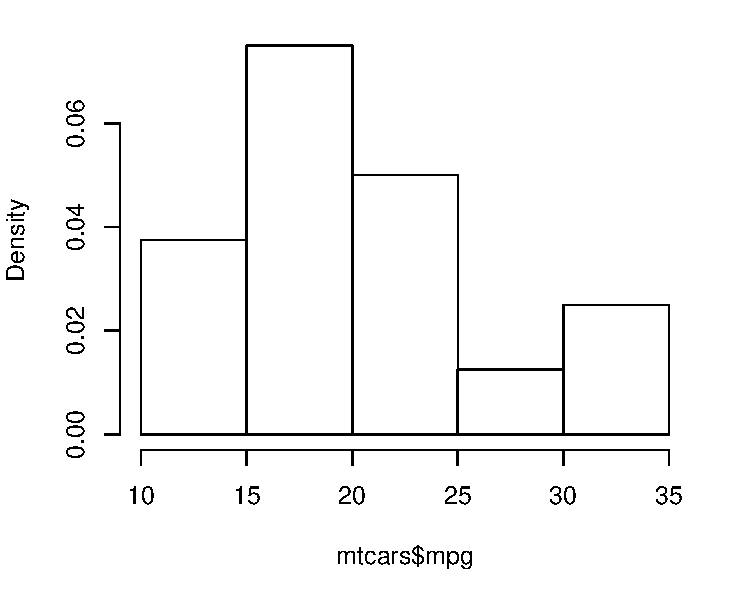
\includegraphics[scale=0.5]{figure/histd_mpg1.pdf}
% \end{figure}
% \end{frame}

%-------------------------------
% \begin{frame}[fragile]
% \begin{verbatim}
% > sort(mtcars$mpg)
%  [1] 10.4 10.4 13.3 14.3 14.7 15.0 15.2 15.2 15.5 15.8 16.4
% [12] 17.3 17.8 18.1 18.7 19.2 19.2 19.7 21.0 21.0 21.4 21.4
% [23] 21.5 22.8 22.8 24.4 26.0 27.3 30.4 30.4 32.4 33.9
% \end{verbatim}
% \vspace{10pt}
% 
% \begin{tabular}{l|lllll}
% Bin ($i$) & $(10, 15]$ & $(15, 20]$ & $(20, 25]$ & $(25, 30]$ & $(30,35]$\\
% \hline
% Count ($f_i$) & 6 & 12 & 8 & 2 & 4\\
% \hline
% Density ($d_i$) & 0.0375 & 0.0750 & 0.0500 & 0.0125  & 0.0250\\
% \end{tabular}
% \vspace{10pt}
% 
% The density values are computed as
% $$d_i = \frac{f_i}{n \Delta x} = \frac{f_i}{32\cdot5},$$
% where $f_i$ is the frequency count for bin $i$, $n$ is the number of observations (e.g., 32 cars), and $\Delta x$ is the bin width (assuming all bins are the same width). For example $6 / (32 \cdot 5) = 0.0375$.\\
% 
% Note that when using density values the area under the histogram is 
% $\sum_{i=1}^{n_b} \Delta x \cdot d_i = 1$, where $n_b$ is the number of bins. 
% \end{frame}

%-------------------------------------------
\begin{frame}[fragile]{Histogram Density Plot}
\small
\begin{itemize}
\item To make a histogram density plot set \texttt{freq=FALSE}
\item When density values are plotted the area under the histogram is 1 (i.e., integrates to 1).  Note that the area under a histogram is computed by summing up the areas of each rectangle (bin widths $\times$ heights)
\item Use \texttt{density()} to superimpose a smooth density curve.
\end{itemize}
\begin{verbatim}
> hist(cdc$weight, freq=FALSE, main='')
> lines(density(cdc$weight), col="red")
\end{verbatim}
\begin{figure}[htbp]
\centering
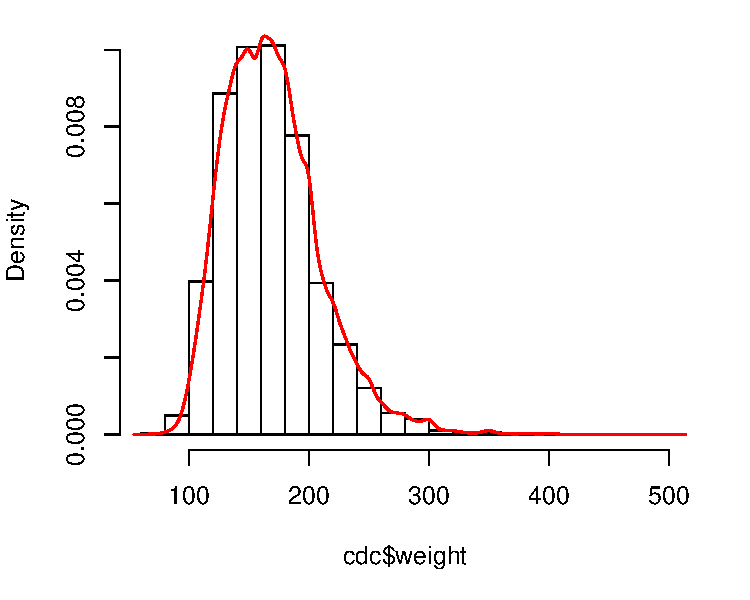
\includegraphics[scale=0.4]{figure/histd_wt.pdf}
\end{figure}
\end{frame}

%-------------------------------------------
\begin{frame}[fragile]{Box Plot}
\begin{verbatim}
> boxplot(cdc$weight, ylab = "Weight")
\end{verbatim}
\begin{figure}[htbp]
\centering
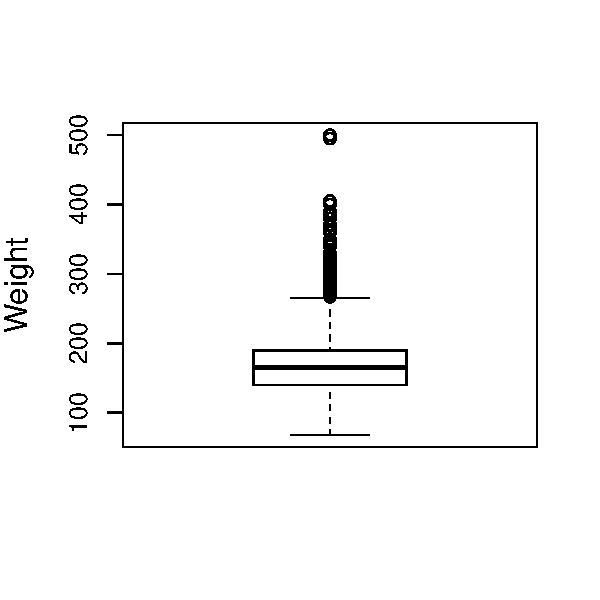
\includegraphics[scale=0.6]{figure/boxplot_wt.pdf}
\end{figure}
\end{frame}

%-------------------------------------------
\begin{frame}[fragile]{Side-by-Side Box Plot}
\small
\begin{verbatim}
> boxplot(weight ~ gender, data=cdc, xlab="Gender", ylab="Weight")
\end{verbatim}
\begin{figure}[htbp]
\centering
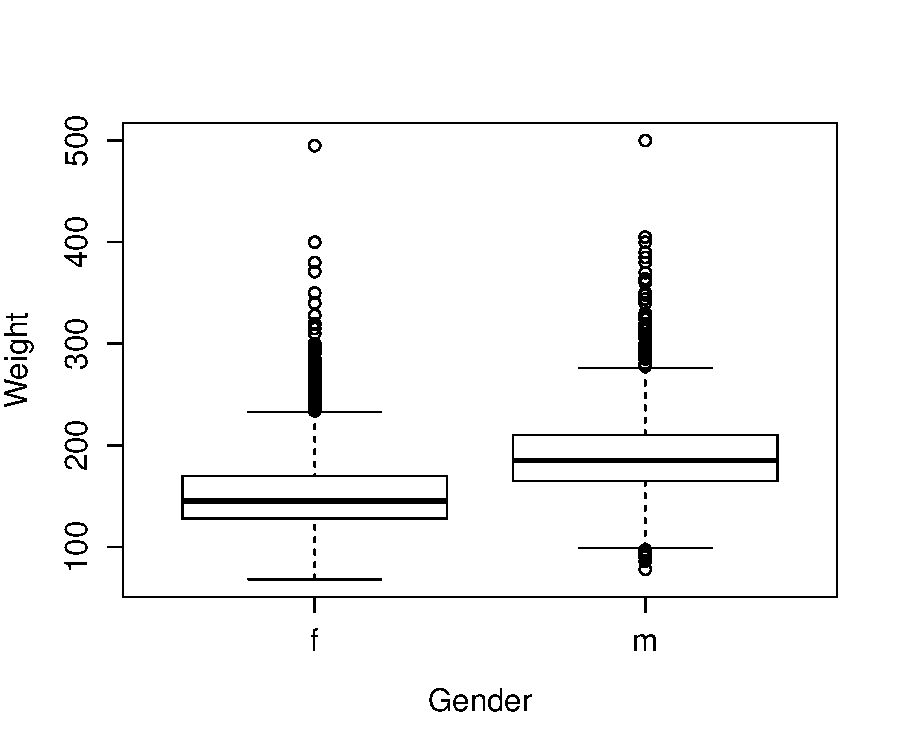
\includegraphics[scale=0.5]{figure/boxplot_wt_mf.pdf}
\end{figure}
\end{frame}

%-------------------------------------------
\begin{frame}[fragile]{Maps}
Use \texttt{library()} to load the \texttt{maps} package into R.\\

\begin{verbatim}
> library(maps) 
> map("world")
\end{verbatim}
\begin{figure}[htbp]
\centering
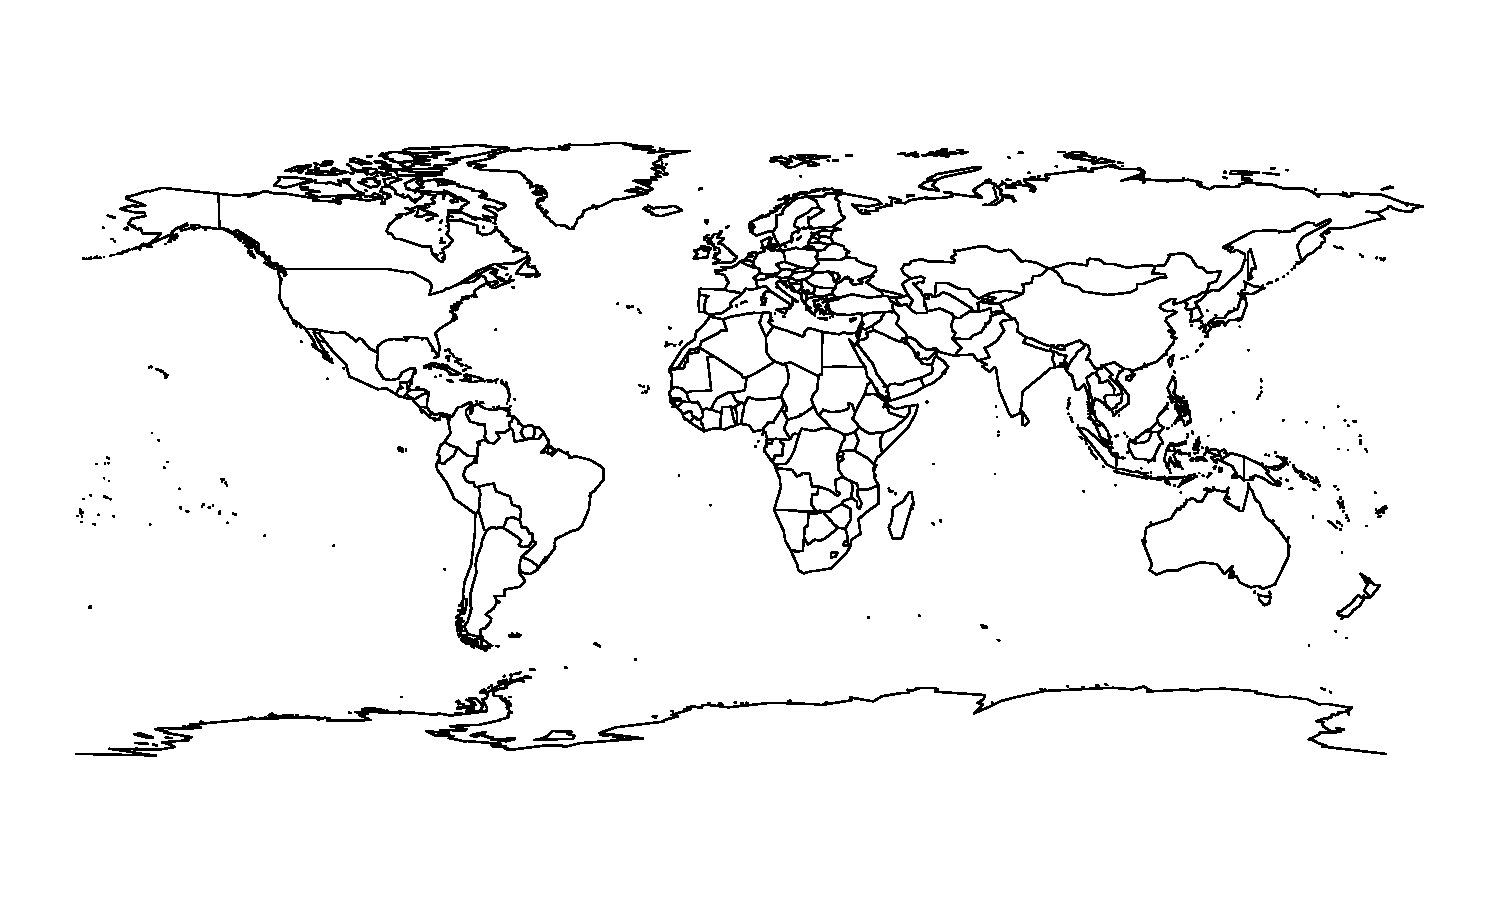
\includegraphics[scale=0.35]{figure/world.pdf}
\end{figure}
 
\end{frame}

%-------------------------------------------
\begin{frame}[fragile]{Maps}
\begin{verbatim}
> map("state", "california")
\end{verbatim}
\begin{figure}[htbp]
\centering
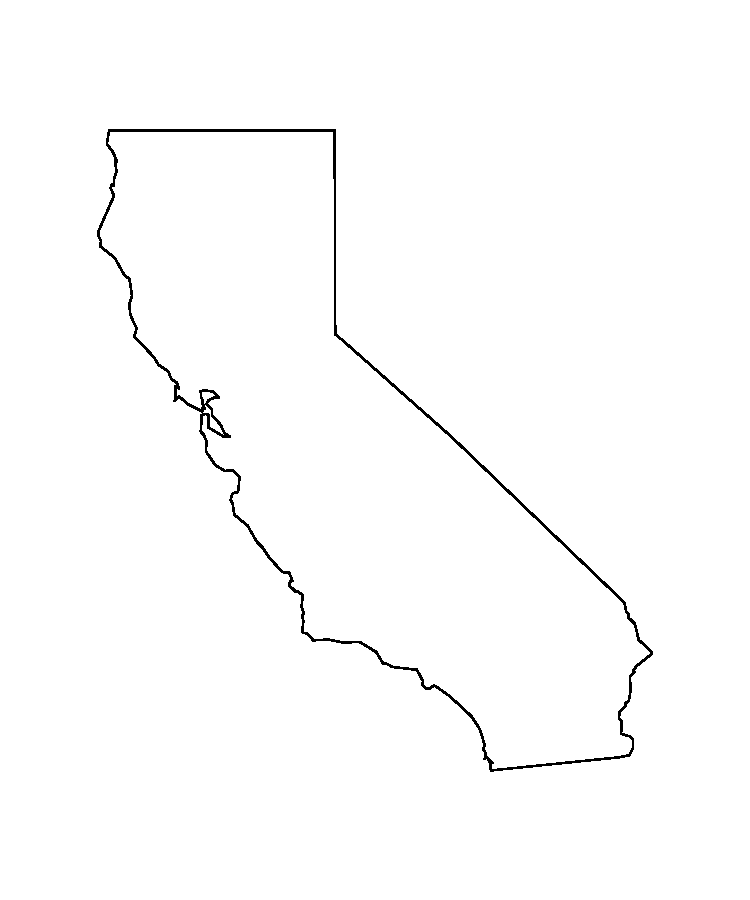
\includegraphics[scale=0.4]{figure/cali.pdf}
\end{figure}
\end{frame}

%-------------------------------------------
\begin{frame}[fragile]{Maps}
\begin{verbatim}
> map("county", "ca")
\end{verbatim}
\begin{figure}[htbp]
\centering
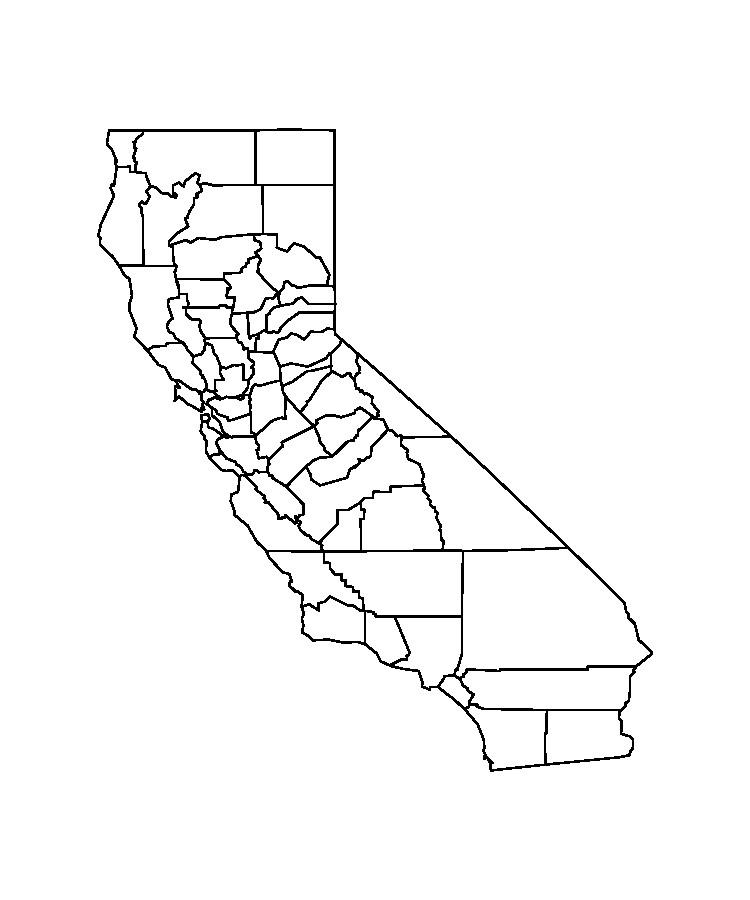
\includegraphics[scale=0.4]{figure/cali2.pdf}
\end{figure}
\end{frame}

%----------------------------------------
\begin{frame}{EPA Stream Data Set}
\begin{itemize}
\item The Environmental Protection Agency (EPA) sampled nearly 2000 stream sites across the conterminous US during the summer months of 2008/09.
\vspace{5pt}
\item This was part of a larger environmental monitoring program called the National Rivers and Stream Assessment (NRSA).
\vspace{5pt}
\item The condition of the stream sites were evaluated as \texttt{Good}, \texttt{Fair}, or \texttt{Poor} according to an aquatic health index. 
\end{itemize}
\end{frame}

%----------------------------------------
\begin{frame}
\begin{figure}[htbp]
\centering

\includegraphics[scale=0.25]{figure/nars_website.png}
\end{figure}
\end{frame}

\begin{frame}[fragile]{EPA Stream Data Set}
\small
\begin{verbatim}
> nrsa <- readRDS(url("https://ericwfox.github.io/data/nrsa.rds"))

> head(nrsa, n=10)
         lon      lat cond
1  -86.88816 33.22342 Poor
2  -86.77562 33.42492 Poor
3  -87.08381 31.67664 Poor
4  -86.32363 33.87273 Good
5  -86.36186 32.99387 Poor
6  -87.73796 34.09180 Poor
7  -85.75963 33.77874 Fair
8  -87.14547 33.35812 Fair
9  -85.61117 34.71586 Poor
10 -87.04203 34.95092 Poor

> dim(nrsa)
[1] 1859    3
\end{verbatim}
\end{frame}

%----------------------------------------
\begin{frame}[fragile]
\small
\begin{verbatim}
> map("state")
> points(nrsa$lon, nrsa$lat, cex=0.5)
\end{verbatim}
\begin{figure}[htbp]
\centering
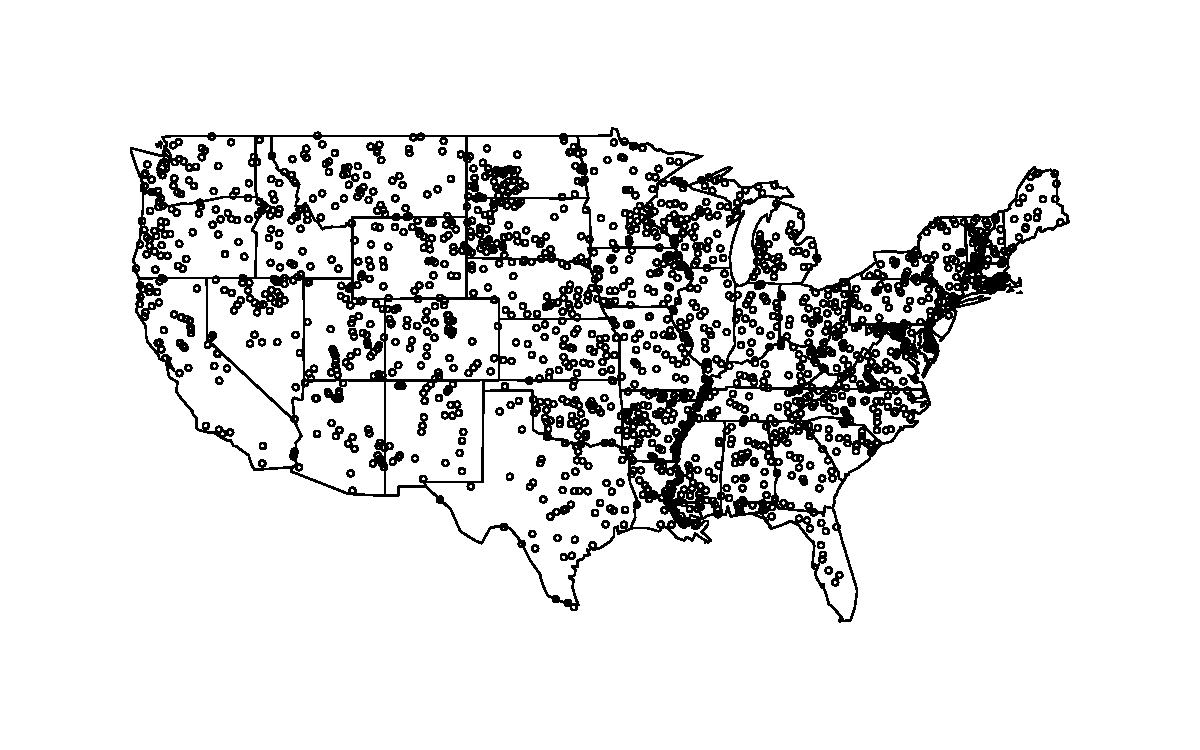
\includegraphics[scale=0.6]{figure/nrsamap0.pdf}
\end{figure}
\end{frame}


%----------------------------------------
\begin{frame}[fragile]
\begin{figure}[htbp]
\centering
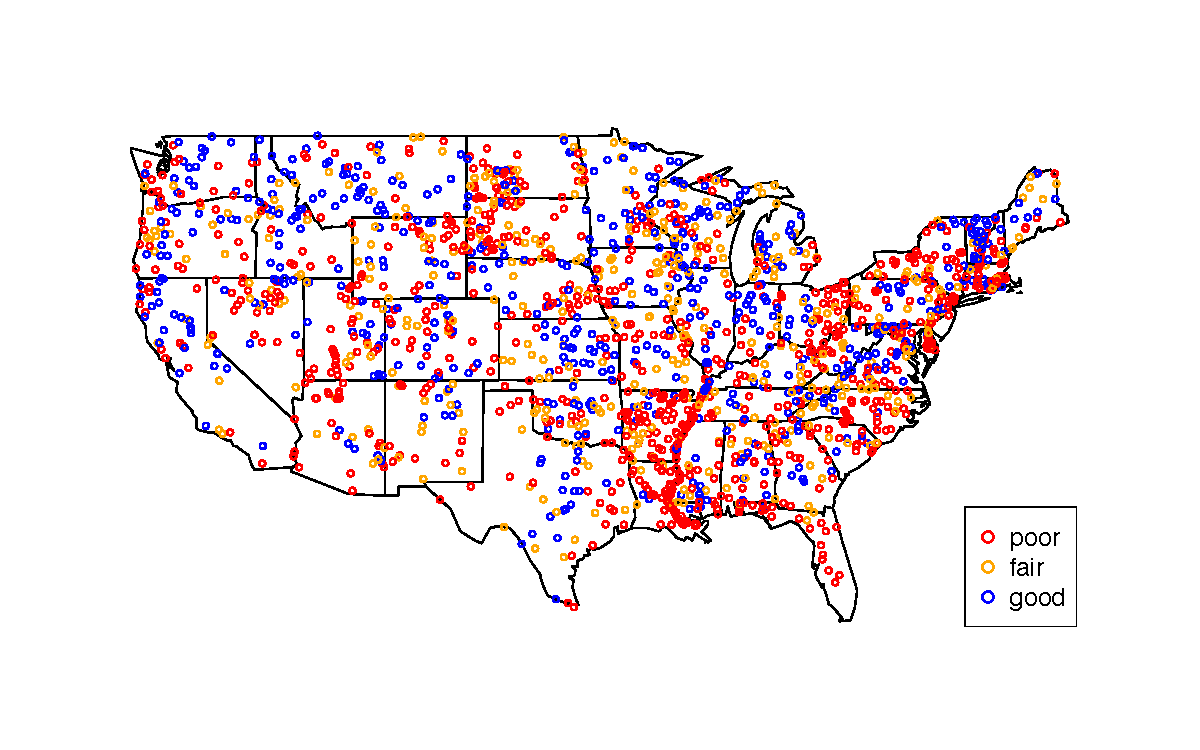
\includegraphics[scale=0.6]{figure/nrsamap.pdf}
\end{figure}
\end{frame}

%----------------------------------------
\begin{frame}[fragile]
Code used to create last map:
\small
\begin{verbatim}
> nrsa_good <- subset(nrsa, cond == "Good")
> nrsa_fair <- subset(nrsa, cond == "Fair")
> nrsa_poor <- subset(nrsa, cond == "Poor")

> map("state")
> points(nrsa_good$lon, nrsa_good$lat, cex=0.5, col = "blue")
> points(nrsa_fair$lon, nrsa_fair$lat, cex=0.5, col = "orange")
> points(nrsa_poor$lon, nrsa_poor$lat, cex=0.5, col = "red")
> legend("bottomright", c("poor", "fair", "good"), 
         col=c("red","orange","blue"), pch=1)
\end{verbatim}
\end{frame}





\end{document}